%%%%%%%%%%%%%%%%%%%%%%%%%%%%%%%%%%%%%%%%%
% Short Sectioned Assignment
% LaTeX Template
% Version 1.0 (5/5/12)
%
% This template has been downloaded from:
% http://www.LaTeXTemplates.com
%
% Original author:
% Frits Wenneker (http://www.howtotex.com)
%
% License:
% CC BY-NC-SA 3.0 (http://creativecommons.org/licenses/by-nc-sa/3.0/)
%
%%%%%%%%%%%%%%%%%%%%%%%%%%%%%%%%%%%%%%%%%

%----------------------------------------------------------------------------------------
%	PACKAGES AND OTHER DOCUMENT CONFIGURATIONS
%----------------------------------------------------------------------------------------

\documentclass[paper=a4, fontsize=11pt]{scrartcl} % A4 paper and 11pt font size

\usepackage[T1]{fontenc} % Use 8-bit encoding that has 256 glyphs
\usepackage{fourier} % Use the Adobe Utopia font for the document - comment this line to return to the LaTeX default
\usepackage[italian]{babel} % English language/hyphenation
\usepackage{amsmath,amsfonts,amsthm} % Math packages
\usepackage{unicode}
\usepackage[utf8x]{inputenc}
\usepackage{lipsum} % Used for inserting dummy 'Lorem ipsum' text into the template
\usepackage{graphicx}
\usepackage{sectsty} % Allows customizing section commands
\allsectionsfont{\centering \normalfont\scshape} % Make all sections centered, the default font and small caps

\usepackage{fancyhdr} % Custom headers and footers
\pagestyle{fancyplain} % Makes all pages in the document conform to the custom headers and footers
\fancyhead{} % No page header - if you want one, create it in the same way as the footers below
\fancyfoot[L]{} % Empty left footer
\fancyfoot[C]{} % Empty center footer
\fancyfoot[R]{\thepage} % Page numbering for right footer
\renewcommand{\headrulewidth}{0pt} % Remove header underlines
\renewcommand{\footrulewidth}{0pt} % Remove footer underlines
\setlength{\headheight}{13.6pt} % Customize the height of the header

\numberwithin{equation}{section} % Number equations within sections (i.e. 1.1, 1.2, 2.1, 2.2 instead of 1, 2, 3, 4)
%\numberwithin{figure}{section} % Number figures within sections (i.e. 1.1, 1.2, 2.1, 2.2 instead of 1, 2, 3, 4)
\numberwithin{table}{section} % Number tables within sections (i.e. 1.1, 1.2, 2.1, 2.2 instead of 1, 2, 3, 4)

\setlength\parindent{0pt} % Removes all indentation from paragraphs - comment this line for an assignment with lots of text

%----------------------------------------------------------------------------------------
%	TITLE SECTION
%----------------------------------------------------------------------------------------

\newcommand{\horrule}[1]{\rule{\linewidth}{#1}} % Create horizontal rule command with 1 argument of height

\title{	
\normalfont \normalsize 
\textsc{Università degli Studi di Palermo}\\
\textsc{Dottorato di Ricerca}\\[25pt] % Your university, school and/or department name(s)
\horrule{0.5pt} \\[0.4cm] % Thin top horizontal rule
\huge \textit{Distributed Misbehaviour Detection} in sistemi multi-robot cooperanti\\ % The assignment title
\horrule{2pt} \\[0.5cm] % Thick bottom horizontal rule
}

\author{Federico Massa} % Your name

\date{\normalsize 21 Agosto 2017} % Today's date or a custom date

\begin{document}
\bibliographystyle{IEEEtran}
\maketitle % Print the title

%----------------------------------------------------------------------------------------
%	INTRO
%----------------------------------------------------------------------------------------

\section{Introduzione}

%DISTRIBUTED
La maggiore disponibilità di risorse computazionali degli ultimi decenni ha causato un crescente interesse verso algoritmi distribuiti in applicazioni robotiche \cite{Lynch-book}. In particolare nell'ambito del Controllo, il cambio di paradigma in questo senso ha reso possibile la cooperazione tra agenti eterogenei, ognuno con
diversi tipi di sensori di bordo, potenza computazionale e attuativa, che, eventualmente avvalendosi di sistemi di comunicazione per lo scambio di informazioni, sono in grado di eseguire insieme un compito assegnato,
incrementando l'efficienza con cui viene svolto \cite{coordination1}. \\

%MULTI-ROBOT
Lo sviluppo di tali algoritmi consente dunque di aprire la strada a ``società'' di robot    \cite{ram10-bfp}, indipendenti e consapevoli della presenza di altri agenti, che possono comunicare tra loro scambiandosi
informazioni sull'ambiente. 
%In generale la capacità di inferenza richiesta per ognuno degli agenti dipende molto dal tipo di ambiente in cui essi devono lavorare e dai vincoli che devono rispettare. 
Ognuno di essi deve rispettare alcune regole
imposte dalla sua appartenenza a tale gruppo, che ne garantiscono il corretto funzionamento nel pieno rispetto dei vincoli imposti dall'ambiente
(un tipico esempio di riguarda la sicurezza necessaria laddove 
sia prevista l'interazione con esseri umani) e dal compito assegnato. 
Come nelle società umane, la cooperazione
può svolgere un ruolo determinante, ed esistono già esempi di questo
tipo nel campo della robotica. Si pensi ad esempio ad un contesto di tipo autostradale in cui 
più veicoli (autonomi o semi-autonomi) si mantengono in formazione di \textit{platoon} (Fig. \ref{img:platoon}), e si coordinano tramite lo scambio di informazioni sensoriali tra vicini \cite{platoon1}, al 
fine di raggiungere in maniera più efficiente la destinazione. \\


%MISBEHAVIOUR - ATTACKS
In questo progetto ci interessiamo a due possibili cause che possono generare
deviazioni (\textit{misbehaviours}) dal comportamento corretto dei robot: la presenza di quelli che 
da ora in poi definiremo \textit{agenti non cooperanti}, ovvero che non seguono (in modo anche parziale) le regole sociali, e
i cyber-attacchi che consistono nella comunicazione (da parte di un agente corrotto), di informazioni scorrette sullo stato del sistema. \\

%DETECTION
In questa ipotesi, diventa dunque importante realizzare dei
sistemi di verifica del comportamento degli agenti. In entrambe le situazioni indesiderate descritte, il processo di rilevamento e della possibile identificazione dell'agente compromesso può difficilmente essere portato a compimento da un singolo agente, a causa del fatto che ognuno può possedere una conoscenza solo parziale dello stato degli altri.
Lo scambio tra gli agenti delle informazioni possedute sull'ambiente circostante può rendere questo problema meglio affrontabile, ma introduce
anche un problema di sicurezza, rendendo possibile che un agente malevolo 
interferisca durante la comunicazione. \\

L'obiettivo principale di questo progetto è 
lo sviluppo di un framework distribuito per la rivelazione di misbehaviours
e di una classe di cyber-attacchi in società multi-robot eterogenee e cooperanti.

\begin{figure}[ht]
\centering
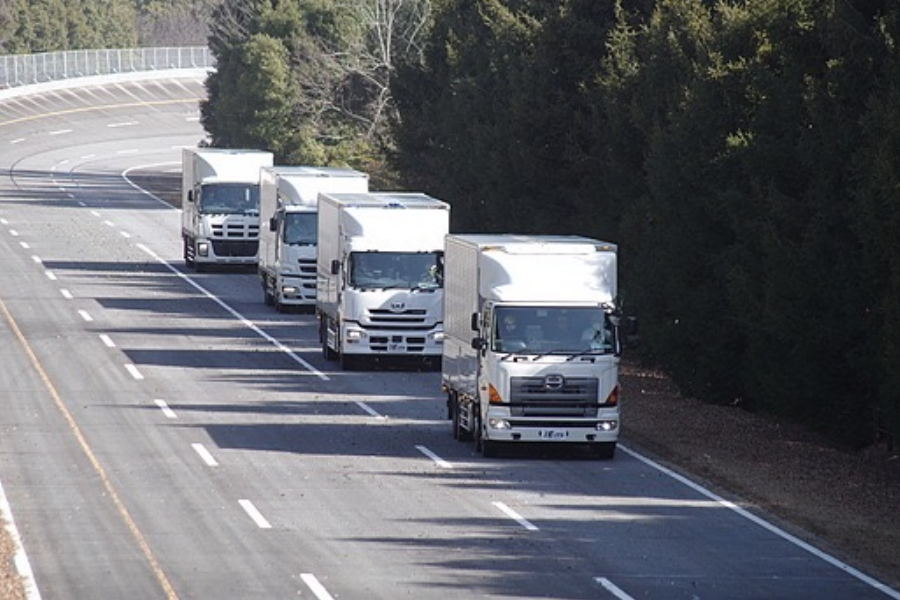
\includegraphics[width=0.5\textwidth]{platoon}
\caption{Esempio di società cooperante: veicoli in formazione di platoon.}
\label{img:platoon}
\end{figure}



%----------------------------------------------------------------------------------------
% 	STATO DELL'ARTE
%----------------------------------------------------------------------------------------
\section{Stato dell'arte}
Il problema della \textit{misbehaviour detection} non è stato ancora molto affrontato
in robotica, mentre si incontra spesso in informatica sotto il nome di \textit{intrusion detection} (ID), dove lo scopo è quello di individuare eventuali attacchi malevoli 
a danno di uno o più nodi della rete \cite{IDS3}\cite{Pasqualetti_attackdetection}. L'architettura di molti algoritmi con 
questo obiettivo è centralizzata: la raccolta dei dati avviene sui singoli nodi, ma l'analisi viene condotta su un solo nodo o su un numero ristretto. Sebbene le applicazioni robotiche presentino delle sostanziali differenze rispetto alle reti informatiche, molti dei concetti sono analoghi, ed è pertanto importante confrontarsi con gli studi di questo tipo. Uno dei problemi comuni dati dalla centralizzazione è il cosiddetto \textit{single point of failure}, ovvero il
fatto che la riuscita di un attacco da parte di un software/agente malevolo sul nodo centrale possa compromettere la sicurezza dell'intero sistema. 
Un altro problema di questo tipo di sistemi è la \textit{scalabilità}, in particolare in quegli ambienti in cui il numero di 
agenti non sia determinabile a priori e può variare nel tempo. \\
%Questi problemi sono mitigati in architetture ibride,
%dette \textit{gerarchiche} \cite{HierarchicalIDS}, in cui diversi nodi applicano localmente un algoritmo di ID, mentre la decisione finale viene eseguita da un nodo centrale che sfrutta le pre-analisi
%condotte localmente. 

Più raramente il tipo di architettura scelta per questi sistemi è \textit{distribuita} \cite{IDS2}. In particolare in contesti robotici, questa risulta essere molto flessibile, e particolarmente adatta per ambienti eterogenei e in cui la \textit{riconfigurabilità} sia 
una qualità importante \cite{ram10-bfp}. Alcuni studi riguardano 
lo sviluppo di un sistema di verifica locale basato sullo studio del moto \cite{misbehDetection}, ma assumono di conoscere il modello dinamico degli
agenti, ipotesi che ai fini di questo progetto è limitante. Per quanto
riguarda gli attacchi è stata già studiata la possibilità di 
riconoscere un agente che invia informazioni scorrette grazie alla comunicazione con gli altri e il raggiungimento di un consenso\cite{commDetection}. 

%----------------------------------------------------------------------------------------
% 	OBIETTIVI PROGETTO
%----------------------------------------------------------------------------------------
\section{Obiettivi del progetto}
Il lavoro che viene proposto riguarda lo sviluppo di un framework per la realizzazione di un Misbehaviour Detection System (MDS) in ambienti robotici eterogenei e cooperanti, con l'obiettivo di rendere il più possibile
semplice la riconfigurazione del sistema. Come già accennato, i tipi di 
comportamento scorretto che vogliamo identificare sono due: 
\begin{itemize}
\item \textit{Agente non cooperante}: un agente che non rispetta le regole della società (potrebbe idealmente far parte di una società diversa o 
essere malfunzionante) \cite{ram10-bfp};
\item \textit{Deceptive attacker}: un agente malevolo o malfunzionante che comunica informazioni
errate agli altri agenti \cite{Pasqualetti_attackdetection}. 
\end{itemize}

Immaginando che il MDS sia installato su uno o più agenti della ``società'' (gli \textit{osservatori}), e che abbia a disposizione 
informazioni
sensoriali adeguate per svolgere tale compito, il
progetto si articola nei passi seguenti:
\begin{description}
\item[Studio dell'ambiente] Durante questa fase preliminare, 
il MDS studia l'ambiente circostante, accumulando tutti i dati
necessari per svolgere correttamente il suo compito. L'elaborazione
di mappe dell'ambiente è un problema molto studiato in robotica \cite{mapping}.

\item[Riconoscimento del comportamento] Il MDS
	costruisce ora, partendo da dati sensoriali di basso livello raccolti 
	in un certo intervallo di tempo, la propria
	conoscenza del comportamento degli agenti combinando informazioni 
	a formare una conoscenza sempre di più alto livello di astrazione. Estendendo questo processo nel tempo
	sarà possibile riconoscere una sequenza di azioni intraprese
	dagli agenti osservati. Per la realizzazione dell'algoritmo
	verranno valutati approcci deterministici e di machine learning, 
	e si cercherà di darne una validazione formale.  
	
\item[Verifica delle regole] Una volta individuate le sequenze di azioni 
	degli agenti osservati ed avendo codificato il sistema di regole
	a priori, è possibile verificare che la sequenza riconosciuta rispetti le regole o meno. In Fig.\ref{img:noright} ne è mostrato un esempio. 
\item[Consenso] A causa della parziale conoscenza degli agenti osservati
dovuta a limiti di portata o accuratezza dei sensori, ostacoli che impediscono
la visione in una certa area e altri, non è sempre possibile il riconoscimento di una particolare azione, quantomeno in maniera efficiente.
Lo scambio di informazioni tra robot e il raggiungimento di un consenso 
sul comportamento possono risolvere il problema \cite{consensus}. Questo, in realtà, 
introduce il problema dell'affidabilità delle informazioni ricevute dagli 
altri agenti.  
\item[Attribuzione di una reputazione] Per mitigare i danni inferti 
da un attaccante \textit{deceptive},
il riconoscimento del comportamento e la verifica delle regole vengono
effettuati dapprima con le sole informazioni possedute dall'osservatore.
Solo successivamente si utilizzano le informazioni possedute dagli altri, le quali vengono valutate e confrontate. Nel caso in cui vi sia una contraddizione tra queste informazioni, un possibile attacco viene rilevato. Studiare come individuare l'attaccante è uno degli obiettivi del progetto. Dalla verifica delle 
regole e l'eventuale consenso, invece, è possibile rilevare gli agenti non cooperanti. Un obiettivo del progetto è anche quello di sviluppare
un sistema di reputazione per gli agenti, in modo che ad ogni azione 
riconosciuta venga attribuito un punteggio basato sulla correttezza o meno
della sua esecuzione. Dopo un tempo sufficiente sarà stato creato 
un profilo dell'agente che ne descrive le caratteristiche comportamentali fondamentali, a disposizione di tutti gli agenti della società affinché possano comportarsi di conseguenza al momento dell'interazione.
\end{description}

\begin{figure}[ht]
\centering
\includegraphics[width=0.5\textwidth]{simulation_01_A03_a}
\caption{Autostrada in cui vige la regola del tenere la corsia più a destra possibile. Un agente non cooperante (00) viene osservato da un altro (03), 
che avendo piena visibilità sulla prima corsia riconosce un comportamento
non conforme alle regole sociali.}
\label{img:noright}
\end{figure}

%----------------------------------------------------------------------------------------
% 	TIMELINE
%----------------------------------------------------------------------------------------
\section{Timeline del progetto}
Il progetto potrà attuarsi nella seguente maniera:
\begin{description}
\item[1° anno]\textbf{- \ Progettazione} \ \\
	1. Definizione del problema e studio delle ricerche già esistenti \\
	2. Individuazione di contesti applicativi adeguati in cui studiare il problema\\
	3. Sviluppo framework di simulazione\\
	4. Sviluppo algoritmi di riconoscimento dei comportamenti
\item[2° anno]\textbf{- \ Test} \ \\
	1. Studio/sviluppo di metodi di codifica delle regole sociali \\
	2. Implementazione e test degli algoritmi all'interno del framework
		di simulazione nei diversi contesti applicativi
\item[3° anno]\textbf{- \ Sperimentazione} \ \\
	1. Individuazione modalità di sperimentazione adeguata, ottimizzando 
	il rapporto tra i costi e l'efficacia con cui l'esperimento dimostra la generalità della soluzione trovata\\
	2. Progettazione dell'esperimento (soluzioni hardware adeguate,
	 complessità dell'ambiente necessaria per ottenere realismo, 
	 ricerca sito dell'esperimento)\\
	3. Installazione del MDS sul robot fisico e test.
	 
\end{description}

\bibliography{project}


\end{document}